\PassOptionsToPackage{unicode=true}{hyperref} % options for packages loaded elsewhere
\PassOptionsToPackage{hyphens}{url}
%
\documentclass[]{article}
\usepackage{lmodern}
\usepackage{amssymb,amsmath}
\usepackage{ifxetex,ifluatex}
\usepackage{fixltx2e} % provides \textsubscript
\ifnum 0\ifxetex 1\fi\ifluatex 1\fi=0 % if pdftex
  \usepackage[T1]{fontenc}
  \usepackage[utf8]{inputenc}
  \usepackage{textcomp} % provides euro and other symbols
\else % if luatex or xelatex
  \usepackage{unicode-math}
  \defaultfontfeatures{Ligatures=TeX,Scale=MatchLowercase}
\fi
% use upquote if available, for straight quotes in verbatim environments
\IfFileExists{upquote.sty}{\usepackage{upquote}}{}
% use microtype if available
\IfFileExists{microtype.sty}{%
\usepackage[]{microtype}
\UseMicrotypeSet[protrusion]{basicmath} % disable protrusion for tt fonts
}{}
\IfFileExists{parskip.sty}{%
\usepackage{parskip}
}{% else
\setlength{\parindent}{0pt}
\setlength{\parskip}{6pt plus 2pt minus 1pt}
}
\usepackage{hyperref}
\hypersetup{
            pdftitle={Supplementary Materials for easyreporting},
            pdfauthor={Dario Righelli; Claudia Angelini},
            pdfborder={0 0 0},
            breaklinks=true}
\urlstyle{same}  % don't use monospace font for urls
\usepackage[margin=1in]{geometry}
\usepackage{color}
\usepackage{fancyvrb}
\newcommand{\VerbBar}{|}
\newcommand{\VERB}{\Verb[commandchars=\\\{\}]}
\DefineVerbatimEnvironment{Highlighting}{Verbatim}{commandchars=\\\{\}}
% Add ',fontsize=\small' for more characters per line
\usepackage{framed}
\definecolor{shadecolor}{RGB}{248,248,248}
\newenvironment{Shaded}{\begin{snugshade}}{\end{snugshade}}
\newcommand{\AlertTok}[1]{\textcolor[rgb]{0.94,0.16,0.16}{#1}}
\newcommand{\AnnotationTok}[1]{\textcolor[rgb]{0.56,0.35,0.01}{\textbf{\textit{#1}}}}
\newcommand{\AttributeTok}[1]{\textcolor[rgb]{0.77,0.63,0.00}{#1}}
\newcommand{\BaseNTok}[1]{\textcolor[rgb]{0.00,0.00,0.81}{#1}}
\newcommand{\BuiltInTok}[1]{#1}
\newcommand{\CharTok}[1]{\textcolor[rgb]{0.31,0.60,0.02}{#1}}
\newcommand{\CommentTok}[1]{\textcolor[rgb]{0.56,0.35,0.01}{\textit{#1}}}
\newcommand{\CommentVarTok}[1]{\textcolor[rgb]{0.56,0.35,0.01}{\textbf{\textit{#1}}}}
\newcommand{\ConstantTok}[1]{\textcolor[rgb]{0.00,0.00,0.00}{#1}}
\newcommand{\ControlFlowTok}[1]{\textcolor[rgb]{0.13,0.29,0.53}{\textbf{#1}}}
\newcommand{\DataTypeTok}[1]{\textcolor[rgb]{0.13,0.29,0.53}{#1}}
\newcommand{\DecValTok}[1]{\textcolor[rgb]{0.00,0.00,0.81}{#1}}
\newcommand{\DocumentationTok}[1]{\textcolor[rgb]{0.56,0.35,0.01}{\textbf{\textit{#1}}}}
\newcommand{\ErrorTok}[1]{\textcolor[rgb]{0.64,0.00,0.00}{\textbf{#1}}}
\newcommand{\ExtensionTok}[1]{#1}
\newcommand{\FloatTok}[1]{\textcolor[rgb]{0.00,0.00,0.81}{#1}}
\newcommand{\FunctionTok}[1]{\textcolor[rgb]{0.00,0.00,0.00}{#1}}
\newcommand{\ImportTok}[1]{#1}
\newcommand{\InformationTok}[1]{\textcolor[rgb]{0.56,0.35,0.01}{\textbf{\textit{#1}}}}
\newcommand{\KeywordTok}[1]{\textcolor[rgb]{0.13,0.29,0.53}{\textbf{#1}}}
\newcommand{\NormalTok}[1]{#1}
\newcommand{\OperatorTok}[1]{\textcolor[rgb]{0.81,0.36,0.00}{\textbf{#1}}}
\newcommand{\OtherTok}[1]{\textcolor[rgb]{0.56,0.35,0.01}{#1}}
\newcommand{\PreprocessorTok}[1]{\textcolor[rgb]{0.56,0.35,0.01}{\textit{#1}}}
\newcommand{\RegionMarkerTok}[1]{#1}
\newcommand{\SpecialCharTok}[1]{\textcolor[rgb]{0.00,0.00,0.00}{#1}}
\newcommand{\SpecialStringTok}[1]{\textcolor[rgb]{0.31,0.60,0.02}{#1}}
\newcommand{\StringTok}[1]{\textcolor[rgb]{0.31,0.60,0.02}{#1}}
\newcommand{\VariableTok}[1]{\textcolor[rgb]{0.00,0.00,0.00}{#1}}
\newcommand{\VerbatimStringTok}[1]{\textcolor[rgb]{0.31,0.60,0.02}{#1}}
\newcommand{\WarningTok}[1]{\textcolor[rgb]{0.56,0.35,0.01}{\textbf{\textit{#1}}}}
\usepackage{graphicx,grffile}
\makeatletter
\def\maxwidth{\ifdim\Gin@nat@width>\linewidth\linewidth\else\Gin@nat@width\fi}
\def\maxheight{\ifdim\Gin@nat@height>\textheight\textheight\else\Gin@nat@height\fi}
\makeatother
% Scale images if necessary, so that they will not overflow the page
% margins by default, and it is still possible to overwrite the defaults
% using explicit options in \includegraphics[width, height, ...]{}
\setkeys{Gin}{width=\maxwidth,height=\maxheight,keepaspectratio}
\setlength{\emergencystretch}{3em}  % prevent overfull lines
\providecommand{\tightlist}{%
  \setlength{\itemsep}{0pt}\setlength{\parskip}{0pt}}
\setcounter{secnumdepth}{5}
% Redefines (sub)paragraphs to behave more like sections
\ifx\paragraph\undefined\else
\let\oldparagraph\paragraph
\renewcommand{\paragraph}[1]{\oldparagraph{#1}\mbox{}}
\fi
\ifx\subparagraph\undefined\else
\let\oldsubparagraph\subparagraph
\renewcommand{\subparagraph}[1]{\oldsubparagraph{#1}\mbox{}}
\fi

% set default figure placement to htbp
\makeatletter
\def\fps@figure{htbp}
\makeatother

\usepackage{etoolbox}
\makeatletter
\providecommand{\subtitle}[1]{% add subtitle to \maketitle
  \apptocmd{\@title}{\par {\large #1 \par}}{}{}
}
\makeatother
\usepackage{float}
\usepackage{caption}

\title{Supplementary Materials for easyreporting}
\providecommand{\subtitle}[1]{}
\subtitle{A Bioconductor package for implementing reproducible research}
\author{Dario Righelli\footnote{Istituto per le Applicazioni del Calcolo ``M.
  Picone'' - Consiglio Nazionale delle Ricerche} \and Claudia Angelini\footnote{Istituto per le Applicazioni del Calcolo ``M.
  Picone'' - Consiglio Nazionale delle Ricerche}}
\date{2020-11-29}

\begin{document}
\maketitle

\newcommand{\beginsupplement}{%
        \setcounter{table}{0}
        \renewcommand{\thetable}{S\arabic{table}}%
        \setcounter{figure}{0}
        \renewcommand{\thefigure}{S\arabic{figure}}%
     }

\hypertarget{abstract}{%
\section{Abstract}\label{abstract}}

\emph{easyreporting} is an R/Bioconductor package developed to
facilitate the implementation of Reproducible Research (RR) inside other
packages/software with requiring low/no knowledge of the R Markdown
language.

More in detail, \emph{easyreporting} is an S4 class that schematically
represents the structure of a R Markdown file. Therefore, with
\emph{easyreporting} an analysis report can be seen as a particular
instance (i.e., R object) of the easyreporting class. A series of
attributes and methods implemented with the class allow the user to
structure the components of the report in the desired way, by adding
titles, document sections, comments, code chunks, and so on (see Table
S1 for the list of attributes and methods). The R object is step-by-step
updated each time a new code chunk is added. At the end of the analysis,
the R object can be compiled to produce the typical HTML report of the
analysis that can be attached to a publication as supplementary
material.

\emph{easyreporting} can be useful in any data analysis project, but it
turns out to be particularly useful in the bioinformatics field, where
the complexity of the analyses makes it extremely difficult to trace all
the steps and parameters used in the data analysis. Moreover,
\emph{easyreporting} can be also used by developers to automatically
trace the analysis steps within Graphical User Interfaces (GUIs).

\hypertarget{general-description}{%
\section{General Description}\label{general-description}}

You can also find additional files of this work at the following link
such as:

\url{https://github.com/drighelli/easyreporting_supplementary}

\begin{itemize}
\tightlist
\item
  this document

  \begin{itemize}
  \tightlist
  \item
    Rmd file
  \item
    Pdf file
  \item
    Tex file (produced by rmakrdown)
  \end{itemize}
\item
  the files needed to produce the report described in our work

  \begin{itemize}
  \tightlist
  \item
    R file with the RNA-seq analysis made using easyreporting
  \item
    Rmd report file produced by easyreporting
  \item
    Pdf file of the Rmd compiled report
  \end{itemize}
\end{itemize}

\hypertarget{package-installation}{%
\subsection{Package Installation}\label{package-installation}}

\emph{easyreporting} is available on Bioconductor since version 3.11
(R\textgreater{}=4.0).

To install it, please execute the following code:

\begin{Shaded}
\begin{Highlighting}[]
\ControlFlowTok{if}\NormalTok{ (}\OperatorTok{!}\KeywordTok{requireNamespace}\NormalTok{(}\StringTok{"BiocManager"}\NormalTok{, }\DataTypeTok{quietly =} \OtherTok{TRUE}\NormalTok{))}
    \KeywordTok{install.packages}\NormalTok{(}\StringTok{"BiocManager"}\NormalTok{)}

\NormalTok{BiocManager}\OperatorTok{::}\KeywordTok{install}\NormalTok{(}\StringTok{"easyreporting"}\NormalTok{)}
\end{Highlighting}
\end{Shaded}

After the package is installed, the user needs to load the
\emph{easyreporting} package into the R workspace by using the following
command

\begin{Shaded}
\begin{Highlighting}[]
\KeywordTok{library}\NormalTok{(}\StringTok{"easyreporting"}\NormalTok{) }
\end{Highlighting}
\end{Shaded}

%
        \setcounter{table}{0}
        \renewcommand{\thetable}{S\arabic{table}}%
        \setcounter{figure}{0}
        \renewcommand{\thefigure}{S\arabic{figure}}%

\hypertarget{easyreporting-accessory-functions}{%
\subsection{Easyreporting Accessory
Functions}\label{easyreporting-accessory-functions}}

Supplementary Table S1 lists the additional accessory functions that can
be easily imported with the \texttt{system.file} as examples of
user-defined functions. Note, these functions do not belong to the
\emph{easyreporting} package, but they are released within the package
as external scripts to show the user how to trace external functions.

\begin{table}
\begin{tabular}{l|l|l}
\hline
\textbf{Functions} & \textbf{Description} & \textbf{Package Location} \\ \hline
importData & wrapper for reading xlsx data file & script/importFunctions.R \\
applyEdgeREx & performs edgeR Differential Expression test & script/geneFunctions.R \\ 
MAedgeRMAPlotEx & shows an MA-plot starting from edgeR results & script/plotFunctions.R \\ 
VolcanoPlot & shows a Volcano-plot starting from edgeR results & script/plotFunctions.R \\ 
traceAndPlotMAPlot & wrapper for tracing and showing the MAedgeRMAPlotEx & script/plotFunctions.R \\ \hline
traceAndPlotVolcano & wrapper for tracing and showing the Volcano plot into the Shiny GUI & shiny\_examples/volcano\_app/server.R \\
server & Shiny GUI server for the Volcano plot examaple & shiny\_examples/volcano\_app/server.R \\
ui & Shiny GUI ui for the Volcano plot examaple & shiny\_examples/volcano\_app/ui.R \\ \hline
\end{tabular}
\caption{Accessory functions released with the *easyreporting* package.}
\end{table}

\hypertarget{easyreporting-bulk-rna-seq-analysis}{%
\section{Easyreporting Bulk RNA-seq
Analysis}\label{easyreporting-bulk-rna-seq-analysis}}

The following sub-sections are organized to offer an example of how
\emph{easyreporting} can be used to create an automatic R Markdown file
describing a given bulk RNA-seq analysis. For the sake of generality, we
divided the analysis in several code chunks (CC) and we used in the CCs
both functions from well-known R packages and user-defined functions.

To perform a complete walkthrough usage example, for each CC, we first
show the \emph{easyreporting} CC (section named ``code side'') with the
R code that is needed to be tracked. Then, the same CC is presented as a
piece of an R Markdown code (section named ``rmarkdown side''). Such a
rmarkdown code is auto produced by the \emph{easyreporting} code side
CC. Then, finally, the third section of the CC shows how the above R
Markdown code appears as a piece of the final report (section named
``report side'').

The shown code has to be meant as illustrative for better understanding
how \emph{easyreporting} can be used to trace code and functions into a
bigger project, such as a GUI for data analysis.

\hypertarget{dataset-description-and-rna-seq-pipeline}{%
\subsection{Dataset Description and RNA-seq
pipeline}\label{dataset-description-and-rna-seq-pipeline}}

As an illustrative purpose, we consider an RNA-seq dataset (GEO
Accession:
\href{https://www.ncbi.nlm.nih.gov/geo/query/acc.cgi?acc=GSE60231}{\emph{GSE60231}})
selected from our previous work on CD8+ dendritic T-cells aimed to
investigate the differences in the immune response of two different
antibodies compared with control.

The dataset contains the raw counts of 37991 genes and is composed of
two replicates for each of the three conditions:

\begin{itemize}
\item
  DEC (fd-scaDEC-205 antibody samples)
\item
  E2 (E2 antibody samples),
\item
  UNTR (control samples)
\end{itemize}

See {[}1{]} for more details.

A typical RNA-seq analysis starts from the mapping of the FASTQ
sequences to a reference genome, followed by the gene expression
quantification of each sample. The quantification step leads to the
so-called raw count matrix, with genes represented on the rows and
samples on the columns, i.e., where each matrix element (i,j) contains
the number of reads of the gene (i) in the sample (j). Such a phase is
the most computationally demanding part and skipped in this example.

For illustrative purposes, here we start the analysis from the raw
counts.\\
The raw count file is released as supplementary data with the
\emph{easyreporting} package (file
\emph{BMDC\_counts\_FeaatureCounts.xlsx}). The illustrated pipeline will
first load the data, perform some diagnostic plots, filter and normalize
the raw count, and visualize the principal component projection. Then,
it will perform differential gene expression analysis and depict the
results in terms of a Venn diagram and MA-plots. Each phase is described
by a specific CC.

The first step requires to initialize the report, then it needs to be
updated each time with a new CC, adding sections and comments when
necessary/possible. At the end of the analysis, the analyst can compile
the final report by using the properly designed method. Each of the
above-mentioned phases the \emph{easyreporting} methods will be used.

\hypertarget{report-initialization}{%
\subsection{Report initialization}\label{report-initialization}}

After loading the \emph{easyreporting} package in the R environment, the
it's necessary to initialize an analysis report by providing the file
name (i.e., ``rnaseq\_report'') and the title of the report (i.e.,
``RNA-seq Analysis Report''). It is also possible to specify an author
(i.e., Dario Righelli).

For simplicity, we set-up a project directory path starting from the
working directory for our report, but other locations can be chosen by
setting the \texttt{file.path} parameter.

The initialization is carried out using the function
\texttt{easyreporting()}. Note that the \texttt{filenamePath} and
\texttt{title} are mandatory parameters, while the \texttt{author} is
optional.

\hypertarget{cc1-code-side}{%
\subsubsection{CC1 code side}\label{cc1-code-side}}

To initialize the report, it can be used the following code

\begin{Shaded}
\begin{Highlighting}[]
\KeywordTok{library}\NormalTok{(}\StringTok{"easyreporting"}\NormalTok{)}
\NormalTok{proj.path <-}\StringTok{ }\KeywordTok{file.path}\NormalTok{(}\KeywordTok{getwd}\NormalTok{(), }\StringTok{"rnaseq_report"}\NormalTok{)}
\NormalTok{bioEr <-}\StringTok{ }\KeywordTok{easyreporting}\NormalTok{(}\DataTypeTok{filenamePath=}\NormalTok{proj.path, }\DataTypeTok{title=}\StringTok{"RNA-seq Analysis Report"}\NormalTok{,}
                       \DataTypeTok{author=}\KeywordTok{c}\NormalTok{(}\StringTok{"Dario Righelli"}\NormalTok{))}
\end{Highlighting}
\end{Shaded}

\hypertarget{cc1-rmarkdown-side}{%
\subsubsection{CC1 rmarkdown side}\label{cc1-rmarkdown-side}}

The above CC1 code initializes the object \emph{bioEr} as an instance of
the \emph{easyreporting} class and produces the following lines of code
that define the header and the options CC inside the
``rnaseq\_report.rmd'' file.

\begin{verbatim}
% ---
%     title: "bioinfo_report"
%     author: "Dario Righelli"
%     date: "2020-11-29"
%     output: rmarkdown::html_document
% ---
% 
% ```{r, include=FALSE}
% knitr::opts_chunk$set(eval=TRUE, echo=TRUE, warning=FALSE, message=FALSE, include=TRUE, cache=TRUE)
% ```
\end{verbatim}

\hypertarget{cc1-report-side}{%
\subsubsection{CC1 report side}\label{cc1-report-side}}

Above CC1 R Markdown side adds into the report the Title, the date time
and the author, and gives instructions for producing the HTML file
format, as shown in Figure S1.

\begin{figure}
\centering
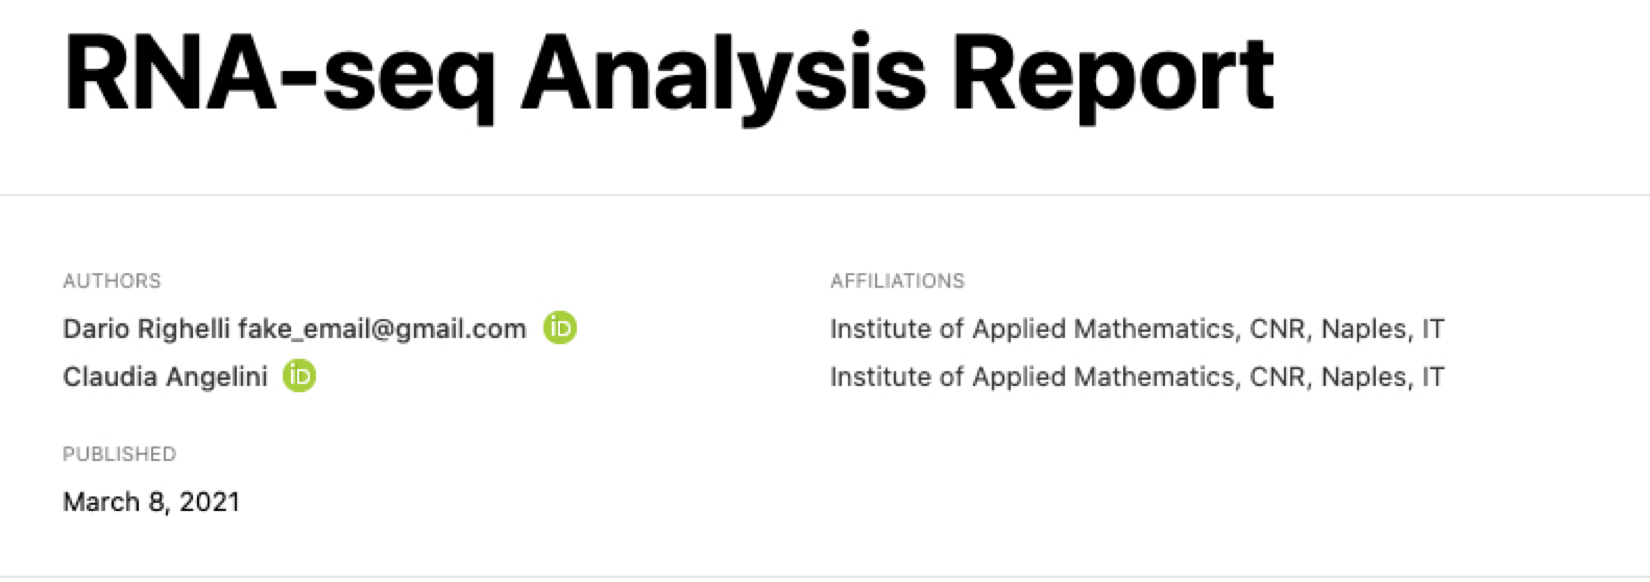
\includegraphics{imgs/1.png}
\caption{The header produced by the CC1 R Markdown side code.}
\end{figure}

\hypertarget{loading-data}{%
\subsection{Loading Data}\label{loading-data}}

Once the report is initialized, it can be added a CC for each step of
the analysis. As mentioned in Section General Description,
\emph{easyreporting} provides two class methods for adding CCs within a
report.

In the first case, it is needed to use the \texttt{mkdCodeChunkSt()} to
open a new CC. Then, to add the code to the markdown, it can be used the
\texttt{mkdVariableAssignment()} and/or the \texttt{mkdGeneralMsg()}
functions, for tracking variables and functions. Finally, the CC can be
closed by using the \texttt{mkdCodeChunkEnd()} function.

In the second approach the\texttt{mkdCodeChunkComplete()} function
allows tracing the steps through the \texttt{message} parameter.

In both cases, it is possible to organize the report in sections, using
the \texttt{mkdTitle()} function. Such operations will be repeated for
each step of the analysis.

Here, we assume that to read the raw counts a user-defined function
named \texttt{importData} is already stored in the
\texttt{importFunctions.R} file available into the package ``script''
folder (see Supplementary Table S1) and we show as illustrative examples
both approaches.

\hypertarget{cc2-code-side}{%
\subsubsection{CC2 code side}\label{cc2-code-side}}

For the sake of illustration, here we use the first approach for adding
the CC. For this purpose, the analyst can use the following code.

\begin{Shaded}
\begin{Highlighting}[]
\KeywordTok{mkdTitle}\NormalTok{(bioEr, }\DataTypeTok{title=}\StringTok{"Loading Counts Data"}\NormalTok{)}
\KeywordTok{mkdCodeChunkSt}\NormalTok{(bioEr, }\DataTypeTok{sourceFilesList=}\KeywordTok{system.file}\NormalTok{(}\StringTok{"script/importFunctions.R"}\NormalTok{, }
                                    \DataTypeTok{package=}\StringTok{"easyreporting"}\NormalTok{), }\DataTypeTok{isComplete=}\OtherTok{TRUE}\NormalTok{)}
\KeywordTok{mkdVariableAssignment}\NormalTok{(bioEr, }\StringTok{"geneCounts"}\NormalTok{, }\KeywordTok{paste}\NormalTok{(}\StringTok{"as.matrix(importData(system.file('"}\NormalTok{,}
                            \StringTok{"extdata/BMDC_counts_FeatureCounts.xlsx', "}\NormalTok{,}
                            \StringTok{"package='easyreporting')))"}\NormalTok{, }\DataTypeTok{sep=}\StringTok{"}\CharTok{\textbackslash{}n}\StringTok{"}\NormalTok{), }\DataTypeTok{show=}\OtherTok{FALSE}\NormalTok{)}
\KeywordTok{mkdGeneralMsg}\NormalTok{(bioEr, }\StringTok{"head(geneCounts, 20)"}\NormalTok{)}
\KeywordTok{mkdCodeChunkEnd}\NormalTok{(bioEr)}
\end{Highlighting}
\end{Shaded}

For comparative purposes, the above code can be replaced by the
following code that implements the second approach.

\begin{Shaded}
\begin{Highlighting}[]
\KeywordTok{mkdCodeChunkComplete}\NormalTok{(}\DataTypeTok{object=}\NormalTok{bioEr, }\DataTypeTok{message=}\KeywordTok{paste}\NormalTok{(}\StringTok{"geneCounts <- "}\NormalTok{,  }
                  \StringTok{"as.matrix(importData(system.file("}\NormalTok{,}
                  \StringTok{"'extdata/BMDC_counts_FeatureCounts.xlsx', "}\NormalTok{, }
                  \StringTok{"package='easyreporting')))"}\NormalTok{, }\StringTok{"head(geneCounts, 20)"}\NormalTok{, }\DataTypeTok{sep=}\StringTok{"}\CharTok{\textbackslash{}n}\StringTok{"}\NormalTok{),}
                  \DataTypeTok{sourceFilesList=}\KeywordTok{system.file}\NormalTok{(}\StringTok{"script/importFunctions.R"}\NormalTok{, }
                  \DataTypeTok{package=}\StringTok{"easyreporting"}\NormalTok{), }
                  \DataTypeTok{optionList=}\KeywordTok{makeOptionsList}\NormalTok{(}\DataTypeTok{evalFlag=}\OtherTok{FALSE}\NormalTok{))}
\end{Highlighting}
\end{Shaded}

Note that the \texttt{mkdCodeChunkComplete} allows also to provide
specific options for the CC which we are creating. In particular, in
this case, we turned the \texttt{evalFlag=FALSE} because we already
processed the step with the previous CC, so the code will not be
evaluated.

\hypertarget{cc2-rmarkdown-side}{%
\subsubsection{CC2 rmarkdown side}\label{cc2-rmarkdown-side}}

The two above CC2 codes add the following CCs in the
``rnaseq\_report.rmd'' file, which are identical. As remarked
previously, the second CC has the \texttt{eval=FALSE} set as its
argument. Moreover, this setting does not affects other global options
of the report.

\begin{verbatim}
 
%# Loading Counts Data
%```{r eval=TRUE, echo=TRUE, warning=FALSE, message=FALSE, include=TRUE, cache=TRUE}
%source("/Library/Frameworks/R.framework/Versions/3.6/
%Resources/library/easyreporting/script/importFunctions.R")
%geneCounts <- as.matrix(importData(system.file('extdata/BMDC_counts_FeatureCounts.xlsx', 
%package='easyreporting')))
%head(geneCounts, 20)
%```
%
%```{r eval=FALSE, echo=TRUE, warning=FALSE, message=FALSE, include=TRUE, cache=TRUE}
%source("/Library/Frameworks/R.framework/Versions/3.6/
%Resources/library/easyreporting/script/importFunctions.R")
%geneCounts <- as.matrix(importData(system.file('extdata/BMDC_counts_FeatureCounts.xlsx', 
%package='easyreporting')))
%head(geneCounts, 20)
%```
\end{verbatim}

\hypertarget{cc2-report-side}{%
\subsubsection{CC2 report side}\label{cc2-report-side}}

The above CC2 code corresponds to the part of the analysis report
depicted in Figure S2.

\begin{figure}[ht]

{\centering 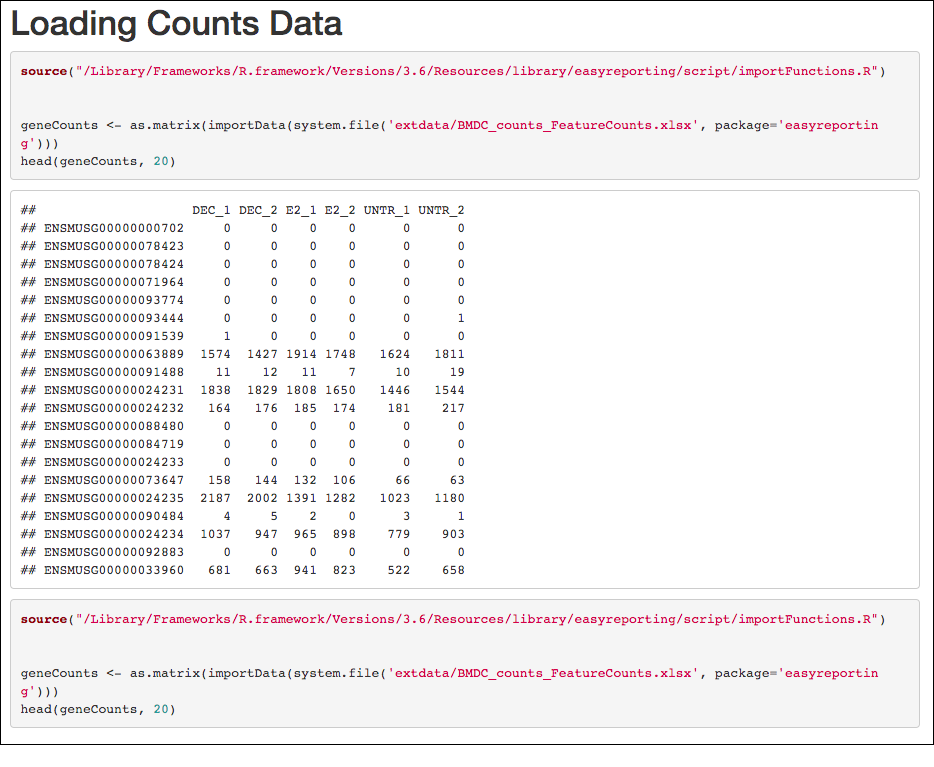
\includegraphics[width=0.95\linewidth]{imgs/21} 

}

\caption{The report section produced by the CC2 R Markdown code}\label{fig:unnamed-chunk-6}
\end{figure}

\hypertarget{data-counts-exploration}{%
\subsection{Data Counts Exploration}\label{data-counts-exploration}}

When analyzing omics data, it is a good practice to visualize a series
of graphs to understand how the samples are distributed and if specific
problems have to be faced during the analysis.

The box-plot of the log-counts is an example of the possible plots that
can be used to compare the distribution of the samples. This plot can be
easily obtained using the R \emph{boxplot} function.

To trace this step in the report, the \texttt{mkdCodeChunkComplete}
function can be used to insert the boxplot function-call as the message
to track in a new CC.

\hypertarget{cc3-code-side}{%
\subsubsection{CC3 code side}\label{cc3-code-side}}

The analyst can use the following code.

\begin{Shaded}
\begin{Highlighting}[]
\KeywordTok{mkdTitle}\NormalTok{(bioEr, }\DataTypeTok{title=}\StringTok{"Plot Boxplot on count data"}\NormalTok{, }\DataTypeTok{level=}\DecValTok{2}\NormalTok{)}
\KeywordTok{mkdCodeChunkComplete}\NormalTok{(bioEr, }\DataTypeTok{message=}\KeywordTok{paste0}\NormalTok{(}\StringTok{"boxplot(log(geneCounts+1),"}\NormalTok{,}
                        \StringTok{" col=c('red','red','orange','orange','purple','purple'),"}\NormalTok{, }
                        \StringTok{" main='Counts BoxPlot',las=1)"}\NormalTok{))}
\end{Highlighting}
\end{Shaded}

\hypertarget{cc3-rmarkdown-side}{%
\subsubsection{CC3 rmarkdown side}\label{cc3-rmarkdown-side}}

The above CC3 code adds the following CC in the ``rnaseq\_report.rmd''
file.

\begin{verbatim}
% ## Plot Boxplot on count data
% ```{r eval=TRUE, echo=TRUE, warning=FALSE, message=FALSE, include=TRUE, cache=TRUE}
% boxplot(log(geneCounts+1), 
% col=c('red','red','orange','orange','purple','purple'), main='Counts BoxPlot',las=1)
% ```
\end{verbatim}

\hypertarget{cc3-report-side}{%
\subsubsection{CC3 report side}\label{cc3-report-side}}

The above CC3 code corresponds to the part of the analysis report
depicted in Figure S3.

\begin{figure}[ht]

{\centering 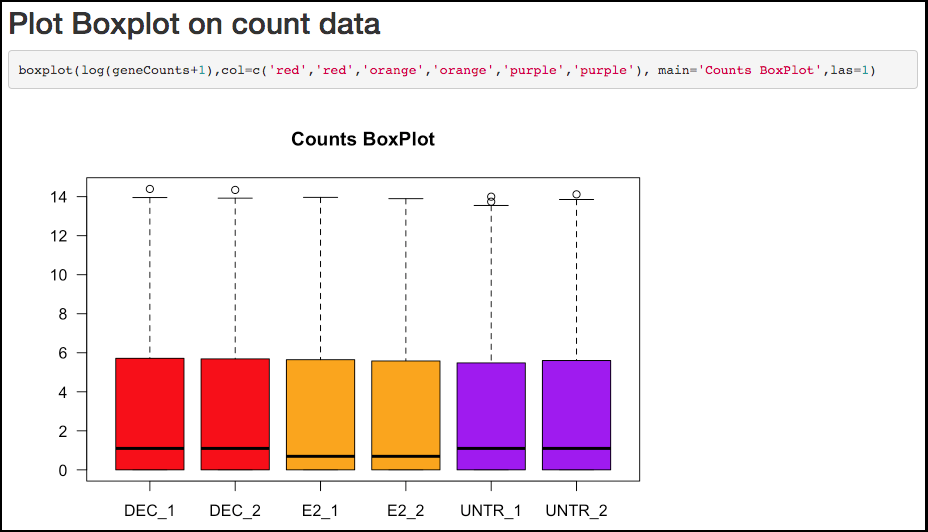
\includegraphics[width=0.95\linewidth]{imgs/3} 

}

\caption{The report section produced by the CC3 R Markdown side code}\label{fig:unnamed-chunk-8}
\end{figure}

In particular, in this case, the figure shows that each sample has a
great number of genes with 0 counts, suggesting that suitable filtering
procedures have to be applied to the data before further processing.

\hypertarget{filtering-and-normalization-steps}{%
\subsection{Filtering and Normalization
steps}\label{filtering-and-normalization-steps}}

To perform the filtering step, we use the \texttt{filtered.data}
function present in the \emph{NOISeq} package. After that, we can
normalize the data across the samples using the
\texttt{betweenLaneNormalization} from the \emph{EDASeq} package and
display the Principal Component Analysis (PCA) by using the
\texttt{plotPCA} function of the \emph{DESeq2} package.

To trace all function calls we need to repeatedly use the
\texttt{mkdCodeChunkComplete} function for consecutive CCs.

\hypertarget{cc4-code-side}{%
\subsubsection{CC4 code side}\label{cc4-code-side}}

The analyst can use the following code.

\begin{Shaded}
\begin{Highlighting}[]
\KeywordTok{mkdTitle}\NormalTok{(bioEr, }\DataTypeTok{title=}\StringTok{"Filtering Low Abundant Features"}\NormalTok{, }\DataTypeTok{level=}\DecValTok{1}\NormalTok{)}
\KeywordTok{mkdCodeChunkComplete}\NormalTok{(}\DataTypeTok{object=}\NormalTok{bioEr, }\DataTypeTok{message=}\KeywordTok{paste}\NormalTok{(}\StringTok{"fgeneCounts <- "}\NormalTok{,}
              \StringTok{"NOISeq::filtered.data(dataset=geneCounts, "}\NormalTok{,}
              \StringTok{"factor=c('D', 'D', 'E', 'E', 'C', 'C'), norm=FALSE, method=3, cv.cutoff=100, cpm=0.5)"}\NormalTok{,}
              \StringTok{"boxplot(log(fgeneCounts+1),col=c('red','red','orange','orange','purple','purple'), "}\NormalTok{,}
              \StringTok{"main='Counts BoxPlot',las=1)"}\NormalTok{, }\DataTypeTok{sep=}\StringTok{"}\CharTok{\textbackslash{}n}\StringTok{"}\NormalTok{))}
\end{Highlighting}
\end{Shaded}

\hypertarget{cc4-rmarkdown-side}{%
\subsubsection{CC4 rmarkdown side}\label{cc4-rmarkdown-side}}

The above CC4 code adds the following CC in the ``rnaseq\_report.rmd''
file.

\begin{verbatim}
% # Filtering Low Abundant Features
% ```{r eval=TRUE, echo=TRUE, warning=FALSE, message=FALSE, include=TRUE, cache=TRUE}
% fgeneCounts <- 
% NOISeq::filtered.data(dataset=geneCounts, 
% factor=c('D', 'D', 'E', 'E', 'C', 'C'), norm=FALSE, method=3, cv.cutoff=100, cpm=0.5)
% boxplot(log(fgeneCounts+1),col=c('red','red','orange','orange','purple','purple'), 
% main='Counts BoxPlot',las=1)
% ```
\end{verbatim}

\hypertarget{cc4-report-side}{%
\subsubsection{CC4 report side}\label{cc4-report-side}}

The above CC4 code corresponds to the part of the analysis report
depicted in Figure S4.

\begin{figure}[ht]

{\centering 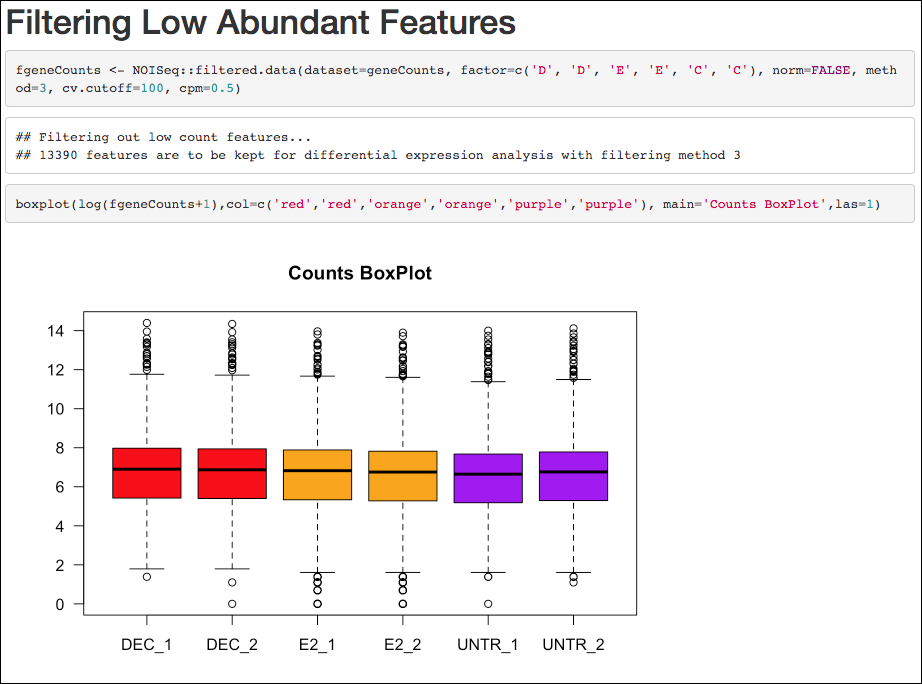
\includegraphics[width=0.9\linewidth]{imgs/4} 

}

\caption{The report section produced by the CC4 R Markdown side code}\label{fig:unnamed-chunk-10}
\end{figure}

\hypertarget{cc5-code-side}{%
\subsubsection{CC5 code side}\label{cc5-code-side}}

For the normalization and the PCA, we implemented the following code.

\begin{Shaded}
\begin{Highlighting}[]
\KeywordTok{mkdTitle}\NormalTok{(bioEr, }\DataTypeTok{title=}\StringTok{"Normalizing Features Across Samples"}\NormalTok{, }\DataTypeTok{level=}\DecValTok{1}\NormalTok{)}
\KeywordTok{mkdCodeChunkComplete}\NormalTok{(}\DataTypeTok{object=}\NormalTok{bioEr, }\DataTypeTok{message=}\KeywordTok{paste}\NormalTok{(}\StringTok{"nfgeneCounts <- "}\NormalTok{,}
              \StringTok{"EDASeq::betweenLaneNormalization(fgeneCounts, which='upper')"}\NormalTok{, }\DataTypeTok{sep=}\StringTok{"}\CharTok{\textbackslash{}n}\StringTok{"}\NormalTok{)}

\KeywordTok{mkdTitle}\NormalTok{(bioEr, }\DataTypeTok{title=}\StringTok{"Plot PCA on count data"}\NormalTok{, }\DataTypeTok{level=}\DecValTok{2}\NormalTok{)}
\KeywordTok{mkdCodeChunkComplete}\NormalTok{(bioEr, }\DataTypeTok{message=}\KeywordTok{paste}\NormalTok{(}\StringTok{"se <- SummarizedExperiment((log2(nfgeneCounts)+ 1), "}\NormalTok{,}
                \StringTok{"colData=DataFrame(rownames=colnames(nfgeneCounts), "}\NormalTok{ ,}
                \StringTok{"condition=c('DEC', 'DEC', 'E2', 'E2', 'CTRL', 'CTRL')))"}\NormalTok{,}
                \StringTok{"DESeq2::plotPCA(DESeqTransform(se))"}\NormalTok{, }\DataTypeTok{sep=}\StringTok{"}\CharTok{\textbackslash{}n}\StringTok{"}\NormalTok{))}
\end{Highlighting}
\end{Shaded}

\hypertarget{cc5-rmarkdown-side}{%
\subsubsection{CC5 rmarkdown side}\label{cc5-rmarkdown-side}}

The above CC5 code adds the following CC in the ``rnaseq\_report.rmd''
file.

\begin{verbatim}
% # Normalizing Features Across Samples
% ```{r eval=TRUE, echo=TRUE, warning=FALSE, message=FALSE, include=TRUE, cache=TRUE}
% nfgeneCounts <- EDASeq::betweenLaneNormalization(fgeneCounts, which='upper')
% ```
% ## Plot PCA on count data
% ```{r eval=TRUE, echo=TRUE, warning=FALSE, message=FALSE, include=TRUE, cache=TRUE}
% 
% se <- SummarizedExperiment((log2(nfgeneCounts)+ 1),
% colData=DataFrame(rownames=colnames(nfgeneCounts), 
% condition=c('DEC', 'DEC', 'E2', 'E2', 'CTRL', 'CTRL')))
% 
% DESeq2::plotPCA(DESeqTransform(se))
% ```
\end{verbatim}

\newpage

\hypertarget{cc5-report-side}{%
\subsubsection{CC5 report side}\label{cc5-report-side}}

The above CC5 code corresponds to the part of the analysis report
depicted in Figure S5.

\begin{figure}[ht]

{\centering 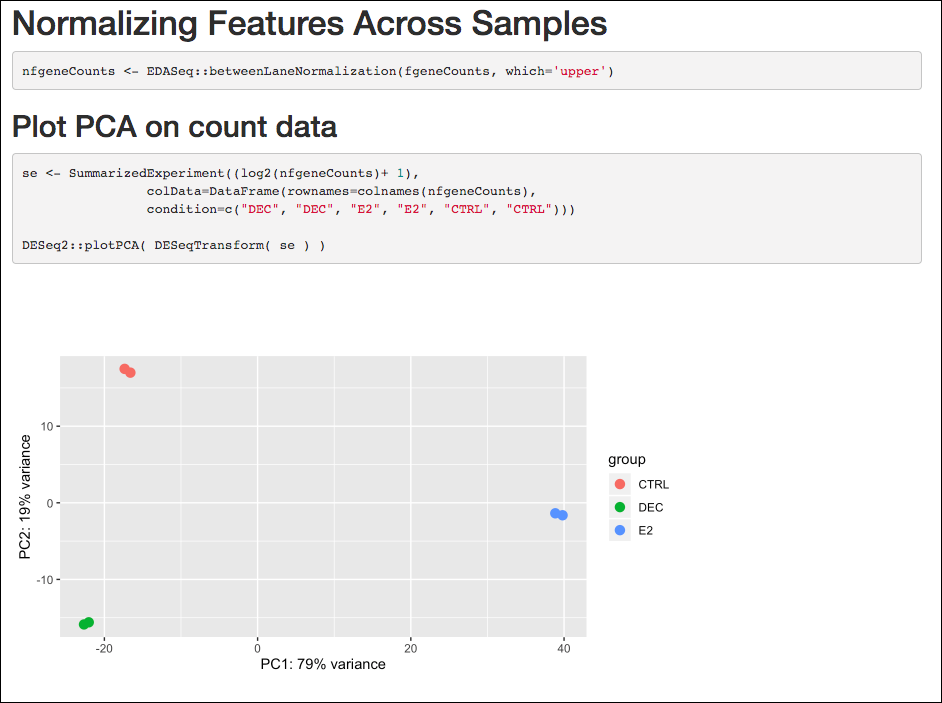
\includegraphics[width=0.9\linewidth]{imgs/5} 

}

\caption{The report section produced by the CC5 R Markdown side code}\label{fig:unnamed-chunk-12}
\end{figure}

In particular, in this case, the figures show that the replicates are
correctly associated and the treatments are correctly grouped. It is
possible to insert comments related to specific outputs as shown in the
following CC.

\hypertarget{differential-expression-analysis}{%
\subsection{Differential Expression
Analysis}\label{differential-expression-analysis}}

Assuming that the data were correctly normalized, it is possible to
perform the differential expression gene (DEG) analysis by using the
\emph{edgeR} package. To simplify such step, we assume to have a
user-defined function named \texttt{applyEdgeREx()} stored in the
\emph{geneFunctions.R} that implements the required test.

Moreover, instead of using the \texttt{mkdCodeChunkComplete()}, here the
\texttt{mkdCodeChunkCommented()} function can be used to allow to add a
comment preceeding the code chunk using the \texttt{commentMsg}
parameter.

For this analysis, we first tested the differences between DEC and
Control, then E2 and Control conditions.

\hypertarget{cc6-code-side}{%
\subsubsection{CC6 code side}\label{cc6-code-side}}

This can be implemented with the following code.

\begin{Shaded}
\begin{Highlighting}[]
\KeywordTok{mkdCodeChunkTitledCommented}\NormalTok{(bioEr, }\DataTypeTok{title=}\StringTok{"Differential Expression Analysis"}\NormalTok{,}
                \DataTypeTok{codeMsg=}\KeywordTok{paste0}\NormalTok{(}\StringTok{"degList <- applyEdgeREx(counts=nfgeneCounts, "}\NormalTok{,}
                \StringTok{"factors=c('DEC', 'DEC', 'E2', 'E2', 'UNTR', 'UNTR'), "}\NormalTok{,}
                \StringTok{"contrasts=c('DEC - UNTR', 'E2 - UNTR'),"}\NormalTok{,}
                \StringTok{"p.threshold=1)"}\NormalTok{),}
            \DataTypeTok{commentMsg=}\KeywordTok{paste}\NormalTok{(}\StringTok{"As we saw from the PCA, the groups are well separated, "}\NormalTok{,}
            \StringTok{"so we can perform a Differential Expression analysis with edgeR."}\NormalTok{, }\DataTypeTok{sep=}\StringTok{"}\CharTok{\textbackslash{}n}\StringTok{"}\NormalTok{),}
            \DataTypeTok{sourceFilesList=}\KeywordTok{system.file}\NormalTok{(}\StringTok{"script/geneFunctions.R"}\NormalTok{, }\DataTypeTok{package=}\StringTok{"easyreporting"}\NormalTok{))}
\end{Highlighting}
\end{Shaded}

\hypertarget{cc6-rmarkdown-side}{%
\subsubsection{CC6 rmarkdown side}\label{cc6-rmarkdown-side}}

The above CC6 code adds the following CC in the ``rnaseq\_report.rmd''
file.

\begin{verbatim}
% # Differential Expression Analysis
% As we saw from the PCA, the groups are well separated, 
% so we can perform a Differential Expression analysis with edgeR.
% ```{r eval=TRUE, echo=TRUE, warning=FALSE, message=FALSE, include=TRUE, cache=TRUE}
% source("/Library/Frameworks/R.framework/Versions/3.6/Resources/library/easyreporting/
% script/geneFunctions.R")
% degList <- applyEdgeREx(counts=nfgeneCounts, 
% factors=c('DEC', 'DEC', 'E2', 'E2', 'UNTR', 'UNTR'), 
% contrasts=c('DEC - UNTR', 'E2 - UNTR'), p.threshold=1)
% ```
\end{verbatim}

\hypertarget{cc6-report-side}{%
\subsubsection{CC6 report side}\label{cc6-report-side}}

The above CC6 code corresponds to the part of the analysis report
depicted in Figure S6.

\begin{figure}[ht]

{\centering 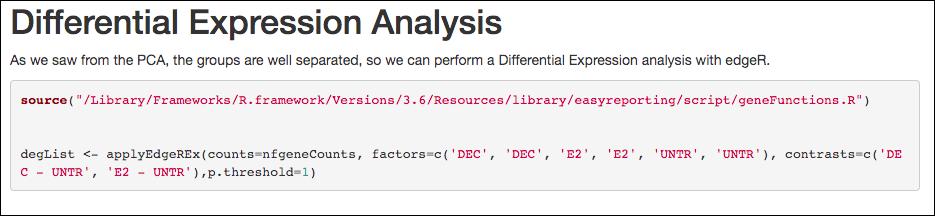
\includegraphics[width=0.95\linewidth]{imgs/6} 

}

\caption{The report section produced by the CC6 R Markdown side code}\label{fig:unnamed-chunk-14}
\end{figure}

\newpage

\hypertarget{differential-expressed-genes-inspection}{%
\subsection{Differential Expressed Genes
Inspection}\label{differential-expressed-genes-inspection}}

The output of a DEG Analysis can be graphically represented by an
MA-plot (or a Volcano plot) for each investigated contrast.

In this example, we can use the MA-plot and produce the graphic by using
the \texttt{plot} function where to depict on the x-axis the log of the
Counts per Million (CPM) and on the y-axis the log of the Fold Change
(FC) computed by \emph{edgeR} during the DEG analysis. In the following
plot, the genes are represented by the dots, in black the not
significant genes and in red the significant DEGs.

With \emph{easyreporting}, by the aid of \texttt{mkdCodeChunkComplete},
it is possible to create a new title and a new chunk within one singular
function-call.

\hypertarget{cc7-code-side}{%
\subsubsection{CC7 code side}\label{cc7-code-side}}

The user can use the following code.

\begin{Shaded}
\begin{Highlighting}[]
\KeywordTok{mkdTitle}\NormalTok{(bioEr, }\StringTok{"MA Plot of DEGs"}\NormalTok{, }\DataTypeTok{level=}\DecValTok{2}\NormalTok{)}
\KeywordTok{mkdCodeChunkComplete}\NormalTok{(bioEr, }\DataTypeTok{message=}\KeywordTok{paste}\NormalTok{(}\StringTok{"for (i in seq_along(degList)) \{ "}\NormalTok{,}
                            \StringTok{"degenes <- degList[[i]]$FDR < 0.01"}\NormalTok{,}
            \StringTok{"with(degList[[i]], plot(logCPM, logFC, pch=16, cex=0.2, "}\NormalTok{,}
            \StringTok{"main=names(degList)[i]))"}\NormalTok{,}
            \StringTok{"with(degList[[i]], points(logCPM[degenes], logFC[degenes], "}\NormalTok{,}
            \StringTok{"col='red', pch=16, cex=0.2))\}"}\NormalTok{, }\DataTypeTok{sep=}\StringTok{"}\CharTok{\textbackslash{}n}\StringTok{"}\NormalTok{))}
\end{Highlighting}
\end{Shaded}

\hypertarget{cc7-rmarkdown-side}{%
\subsubsection{CC7 rmarkdown side}\label{cc7-rmarkdown-side}}

The above CC7 code adds the following CC in the ``rnaseq\_report.rmd''
file.

\begin{verbatim}
% ## MA Plot of DEGs
% ```{r eval=TRUE, echo=TRUE, warning=FALSE, message=FALSE, include=TRUE, cache=TRUE}
% for (i in seq_along(degList)) { degenes <- degList[[i]]$FDR < 0.01
% with(degList[[i]], plot(logCPM, logFC, pch=16, cex=0.2, main=names(degList)[i]))
% with(degList[[i]], points(logCPM[degenes], logFC[degenes], col='red', pch=16, cex=0.2))}
% ```
\end{verbatim}

\newpage

\hypertarget{cc7-report-side}{%
\subsubsection{CC7 report side}\label{cc7-report-side}}

The above CC7 code corresponds to the part of the analysis report
depicted in Figure S7.

\begin{figure}[ht]

{\centering 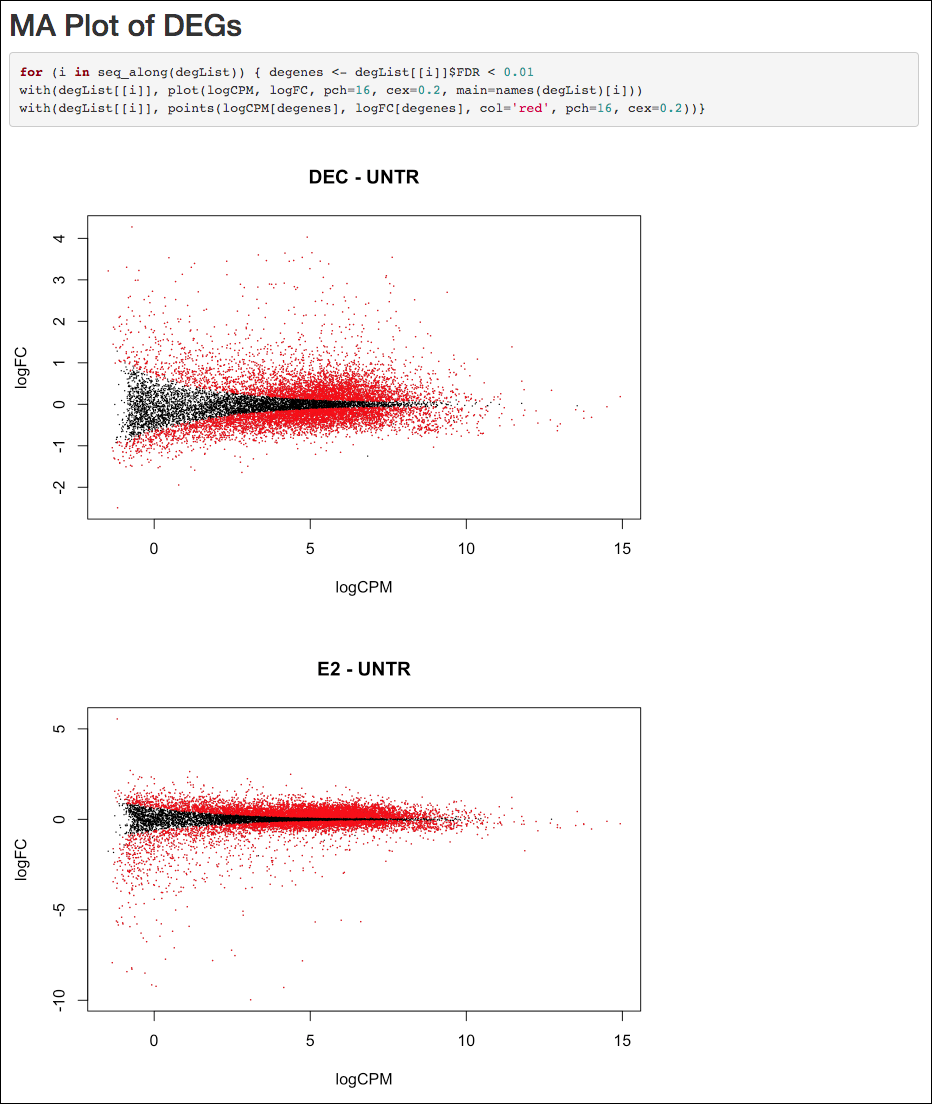
\includegraphics[width=0.7\linewidth]{imgs/7} 

}

\caption{The report section produced by the CC7 R Markdown side code}\label{fig:unnamed-chunk-16}
\end{figure}

\hypertarget{degs-comparison}{%
\subsection{DEGs Comparison}\label{degs-comparison}}

To compare the DEGs between the two main conditions (DEC and E2) we can
use a Venn Diagram, where each circle corresponds to the differentially
expressed genes of a specific comparison.

\hypertarget{cc8-code-side}{%
\subsubsection{CC8 code side}\label{cc8-code-side}}

The user can use the following code.

\begin{Shaded}
\begin{Highlighting}[]
\KeywordTok{mkdTitle}\NormalTok{(bioEr, }\StringTok{"DEGs Venn Diagram"}\NormalTok{, }\DataTypeTok{level=}\DecValTok{2}\NormalTok{)}
\KeywordTok{mkdCodeChunkComplete}\NormalTok{(bioEr, }\DataTypeTok{message=}\KeywordTok{paste}\NormalTok{(}\StringTok{"limma::vennDiagram("}\NormalTok{,}
                  \StringTok{"limma::vennCounts(cbind(degList[[1]]$FDR < 0.01, "}\NormalTok{,}
                  \StringTok{"degList[[2]]$FDR < 0.01)), names=c('DEC', 'E2'))"}\NormalTok{,}\DataTypeTok{sep=}\StringTok{"}\CharTok{\textbackslash{}n}\StringTok{"}\NormalTok{))}
\end{Highlighting}
\end{Shaded}

\hypertarget{cc8-rmarkdown-side}{%
\subsubsection{CC8 rmarkdown side}\label{cc8-rmarkdown-side}}

The above CC8 code adds the following CC in the ``rnaseq\_report.rmd''
file.

\begin{verbatim}
% ### DEGs Venn Diagram
% ```{r eval=TRUE, echo=TRUE, warning=FALSE, message=FALSE, include=TRUE, cache=TRUE}
% limma::vennDiagram(limma::vennCounts(
% cbind(degList[[1]]$FDR < 0.01, degList[[2]]$FDR < 0.01)), names=c('DEC', 'E2'))
% ```
\end{verbatim}

\hypertarget{cc8-report-side}{%
\subsubsection{CC8 report side}\label{cc8-report-side}}

The above CC8 code corresponds to the part of the analysis report
depicted in Figure S8.

\begin{figure}[ht]

{\centering 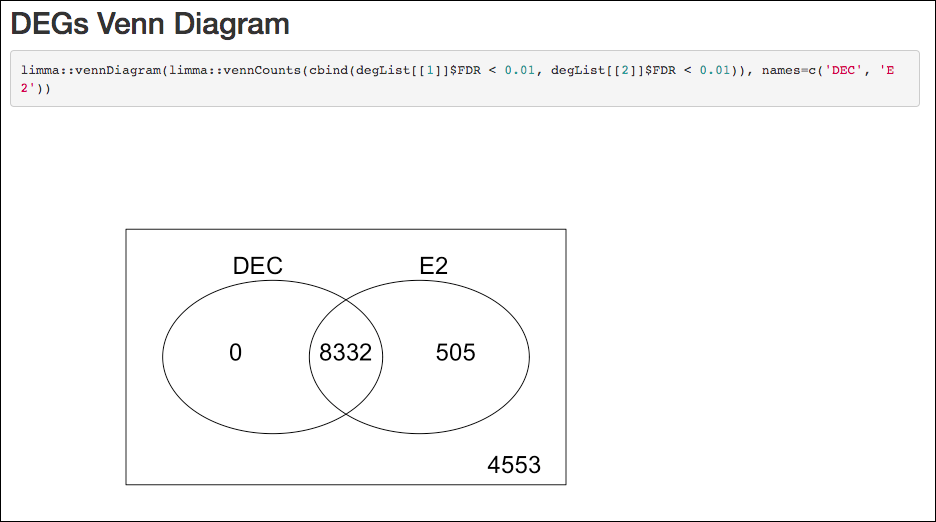
\includegraphics[width=0.95\linewidth]{imgs/8} 

}

\caption{The report section produced by the CC8 R Markdown side code}\label{fig:unnamed-chunk-18}
\end{figure}

\hypertarget{report-compilation}{%
\subsection{Report Compilation}\label{report-compilation}}

Once the analysis is completed, tha package allows to compile the
produced ``rnaseq\_report.rmd'' report simply by using the
\texttt{compile()} method. The \texttt{compile} method produces the
final report (in HTML format) and automatically appends to the report
end a CC with the sessionInfo() to trace all the package versions used
for the analysis.

\hypertarget{cc9-code-side}{%
\subsubsection{CC9 code side}\label{cc9-code-side}}

To compile the report, the analyst can use the following code.

\begin{Shaded}
\begin{Highlighting}[]
\KeywordTok{compile}\NormalTok{(bioEr)}
\end{Highlighting}
\end{Shaded}

\newpage

\hypertarget{cc9-rmarkdown-side}{%
\subsubsection{CC9 rmarkdown side}\label{cc9-rmarkdown-side}}

The above CC9 code adds the following CC in the ``rnaseq\_report.rmd''
file.

\begin{verbatim}
% # Session Info
% 
% ```{r eval=TRUE, echo=TRUE, warning=FALSE, message=FALSE, include=TRUE, cache=TRUE}
% sessionInfo()
% ```
\end{verbatim}

\hypertarget{cc9-report-side}{%
\subsubsection{CC9 report side}\label{cc9-report-side}}

The above CC9 code compiles the entire report and automatically adds at
the end of the report a Session Info section as in the example in Figure
S9.

\begin{figure}[ht]

{\centering 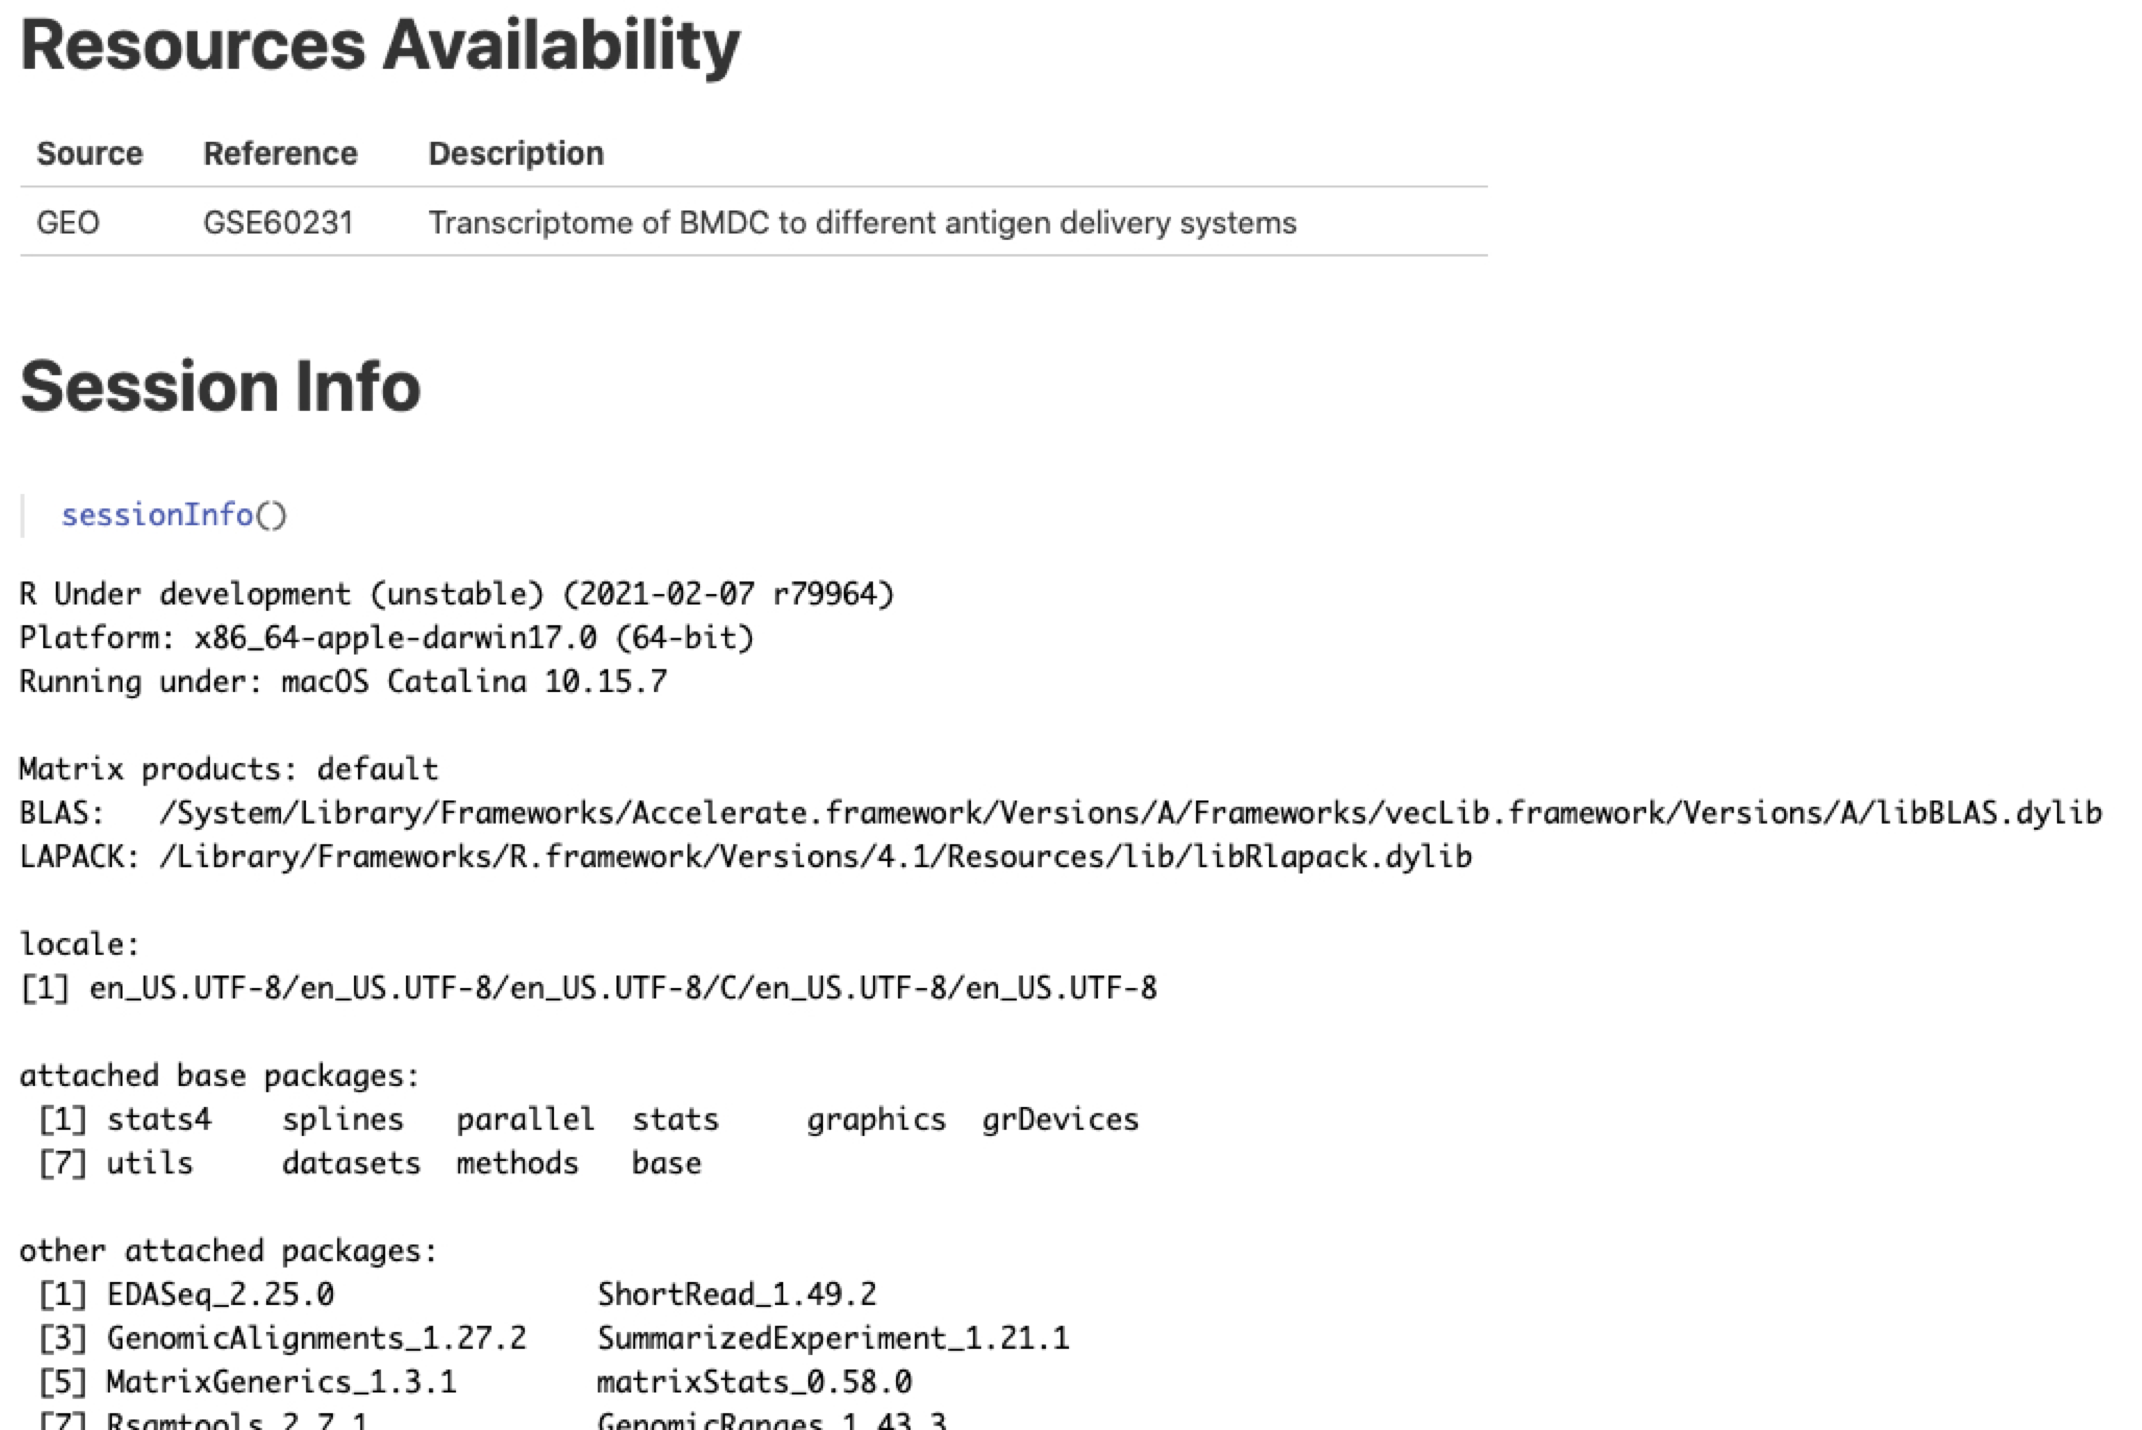
\includegraphics[width=0.95\linewidth]{imgs/9} 

}

\caption{The report section produced by the CC9 R Markdown side code}\label{fig:unnamed-chunk-20}
\end{figure}

\hypertarget{running-easyreporting-example-gui}{%
\section{Running easyreporting example
GUI}\label{running-easyreporting-example-gui}}

To provide an example of GUI that incorporates the \emph{easyreporting}
package, we defined one of them into the package since its version
1.3.1.

To run it just run the following code:

\begin{Shaded}
\begin{Highlighting}[]
\KeywordTok{erGUIVolcano}\NormalTok{()}
\end{Highlighting}
\end{Shaded}

\hypertarget{references}{%
\subsection{References}\label{references}}

\begin{enumerate}
\def\labelenumi{\arabic{enumi}.}
\tightlist
\item
  Costa, V., Righelli, D., Russo, F., De Berardinis, P., Angelini, C.,
  \& D'Apice, L. (2017). Distinct antigen delivery systems induce
  dendritic cells' divergent transcriptional response: new insights from
  a comparative and reproducible computational analysis. International
  journal of molecular sciences, 18(3), 494.
\end{enumerate}

\end{document}
